\documentclass[11  pt]{article} 
\usepackage[lmargin=1in,rmargin=1.75in,bmargin=1in,tmargin=1in]{geometry}  


% For hyperlinking everything
\usepackage{hyperref}
\hypersetup{
	colorlinks=true, %set true if you want colored links
	linktoc=all,     %set to all if you want both sections and subsections linked
	linkcolor=blue,  %choose some color if you want links to stand out
}


\usepackage[latin1]{inputenc}
\usepackage{amsmath}
\usepackage{mathrsfs}  
\usepackage{amsfonts}
\usepackage{amssymb}
\usepackage{graphicx}
\usepackage{subfig}
\usepackage{caption}
\usepackage{algorithm}
%\usepackage{algcompatible}
%\usepackage{algorithmicx}
\usepackage{algpseudocode}

\usepackage{titlesec}
\titleformat{\section}{\fontfamily{lmss}\fontsize{14}{15}\bfseries}{\thesection}{1em}{}
\titleformat{\subsection}{\fontfamily{lmss}\fontsize{12}{15}\bfseries}{\thesubsection}{1em}{}




\usepackage{amsthm}

\newtheoremstyle{noit}
{10pt}% <Space above>
{10pt}% <Space below>
{}% <Body font>
{}% <Indent amount>
{\bfseries}% <Theorem head font>
{.}% <Punctuation after theorem head>
{.5em}% <Space after theorem headi>
{}% <Theorem head spec (can be left empty, meaning `normal')>

\newtheoremstyle{example}
{10pt}% <Space above>
{10pt}% <Space below>
{}% <Body font>
{20pt}% <Indent amount>
{\bfseries}% <Theorem head font>
{.}% <Punctuation after theorem head>
{.5em}% <Space after theorem headi>
{}% <Theorem head spec (can be left empty, meaning `normal')>


\newtheoremstyle{indented}{20pt}{20pt}{\addtolength{\leftskip}{2.5em}}{}{\bfseries}{.}{.5em}{}


\newtheorem{theorem}{Theorem}
\numberwithin{theorem}{section}
\newtheorem{lemma}[theorem]{Lemma}
\newtheorem{corollary}[theorem]{Corollary}
\newtheorem{observation}{Observation}
%\numberwithin{observation}{section}
%\numberwithin{definition}{section}
\newtheorem{conjecture}{Conjecture}
\newtheorem{Qu}{Question}
\newcommand{\QU}{\begin{Qu}\normalfont}

\theoremstyle{noit}
\newtheorem{fact}{Fact}
\newtheorem{definition}{Definition}

\theoremstyle{indented}
\newtheorem{example}{Example}

\theoremstyle{indented}
\newtheorem{problem}{Problem}


%\newenvironment{proof}{\noindent{\bf Proof:} \hspace*{1em}}{
%    \hspace*{\fill} $\Box$ }
%\newenvironment{proof_of}[1]{\noindent {\bf Proof of #1:}
%    \hspace*{1em} }{\hspace*{\fill} $\Box$ }
%\newenvironment{proof_claim}{\begin{quotation} \noindent}{
%    \hspace*{\fill} $\diamond$ \end{quotation}}
\newcommand{\vs}[1]{\vspace{#1}}

\newcommand{\lecture}[2]{
 \noindent
\begin{center}
	\framebox{
		\vbox{
			\hbox to 5.78in { {\bf CSCE 411: Design and Analysis of Algorithms} \hfill  }
			\vspace{2mm}
			\hbox to 5.78in { {\Large \hfill Lecture #1\hfill} }
			\vspace{2mm}
			\hbox to 5.78in { {\it Date: #2 \hfill Lecturer: Nate Veldt} }
		}
	}
\end{center}
\vspace*{4mm}
}


\newcommand{\hw}[2]{
	\noindent
	\begin{center}
		\framebox{
			\vbox{
				\hbox to 5.78in { {\bf CSCE 411: Design and Analysis of Algorithms} \hfill  }
				\vspace{2mm}
				\hbox to 5.78in { {\Large \hfill Homework #1\hfill} }
				\vspace{2mm}
				\hbox to 5.78in { {\it Due date: #2 \hfil} }
			}
		}
	\end{center}
	\vspace*{4mm}
}



\newcommand{\under}[1]{\underline{\hspace{#1}}}
\setlength{\parindent}{0em}

%\usepackage[tagged]{accessibility}

% Graph terms
\newcommand{\vol}{\textbf{vol}}
\newcommand{\cut}{\textbf{cut}}


% Matrices
\newcommand{\mA}{\textbf{A}}
\newcommand{\mB}{\textbf{B}}

% vectors
\newcommand{\ve}{\textbf{e}}
\newcommand{\vx}{\textbf{x}}


% Other
\newcommand{\calN}{\mathcal{N}}

\usepackage{mathtools}
\DeclarePairedDelimiter\ceil{\lceil}{\rceil}
\DeclarePairedDelimiter\floor{\lfloor}{\rfloor}


\newcommand*{\aitem}{ \item[{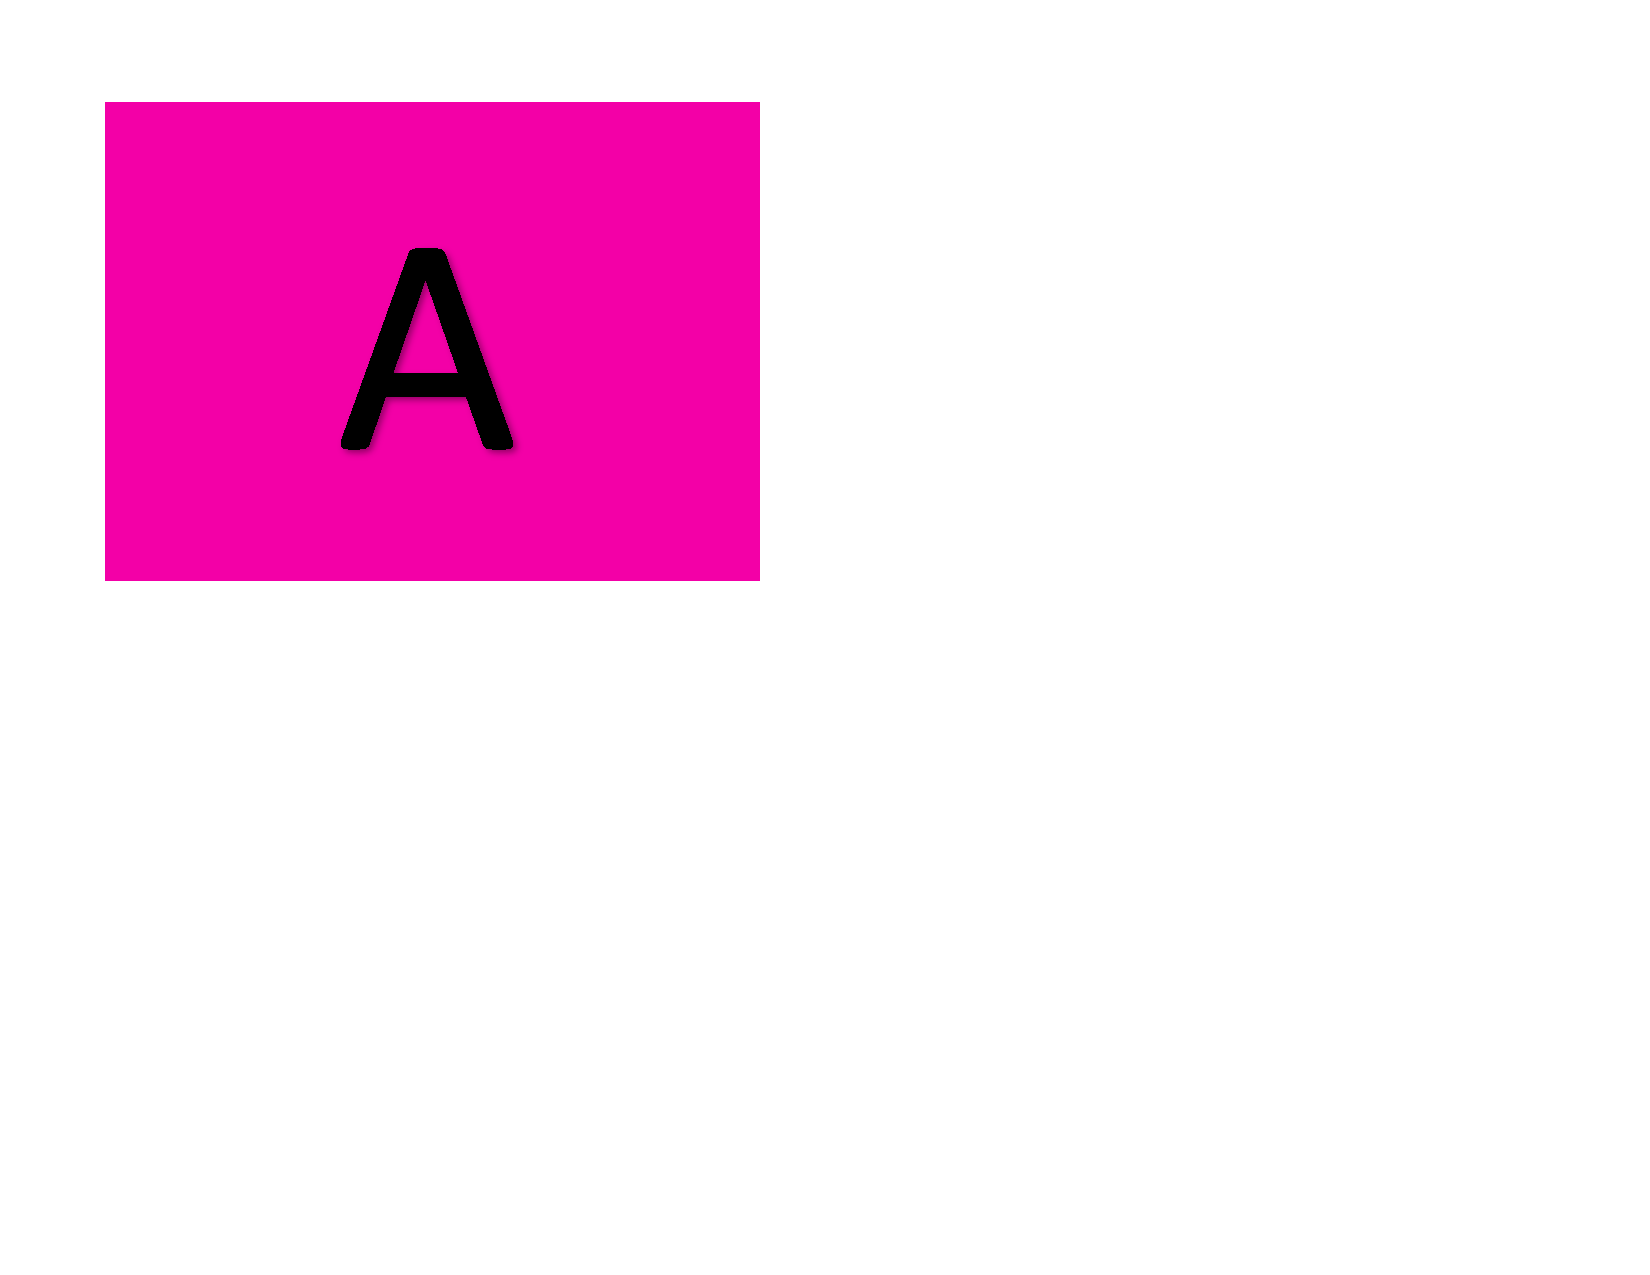
\includegraphics[width=0.8cm,height=0.5cm]{../../Lectures/figures/A}} ]  }
\newcommand*{\bitem}{ \item[{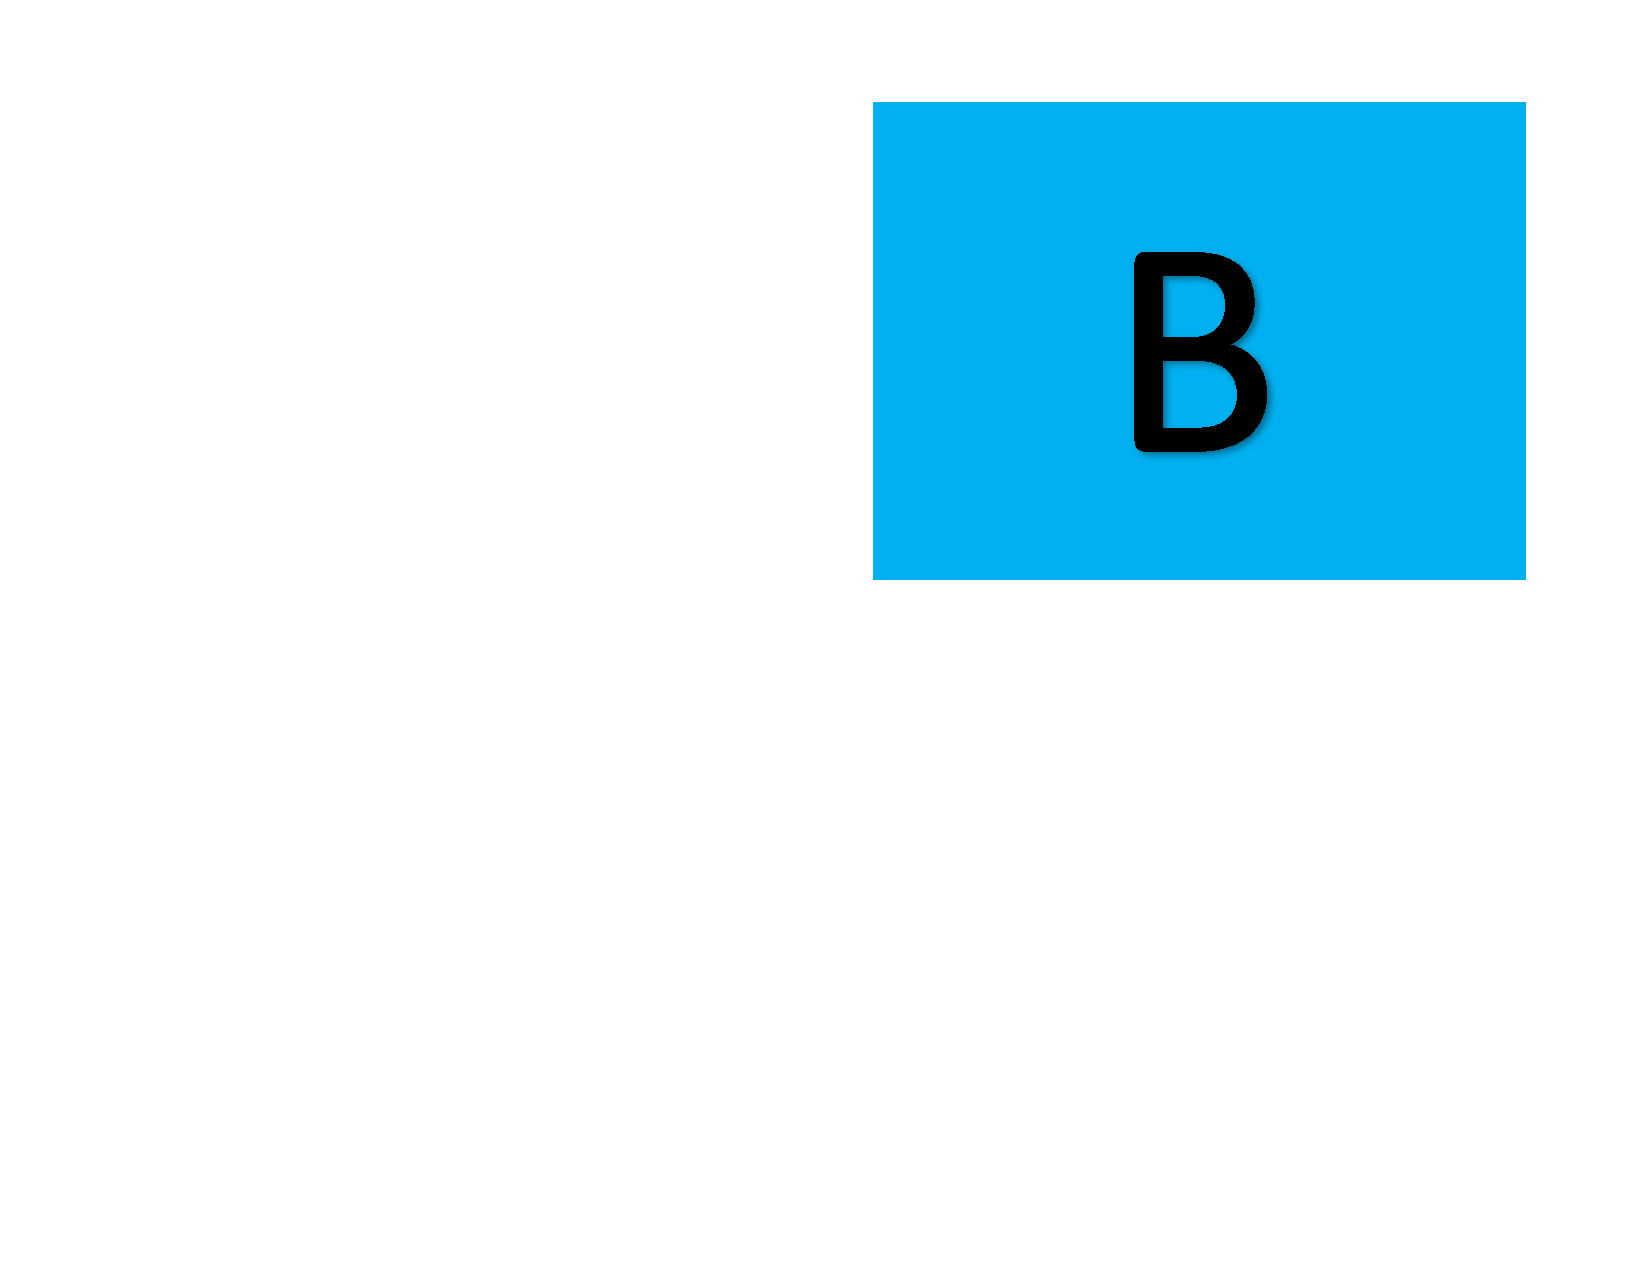
\includegraphics[width=0.8cm,height=0.5cm]{../../Lectures/figures/B}} ]  }
\newcommand*{\citem}{ \item[{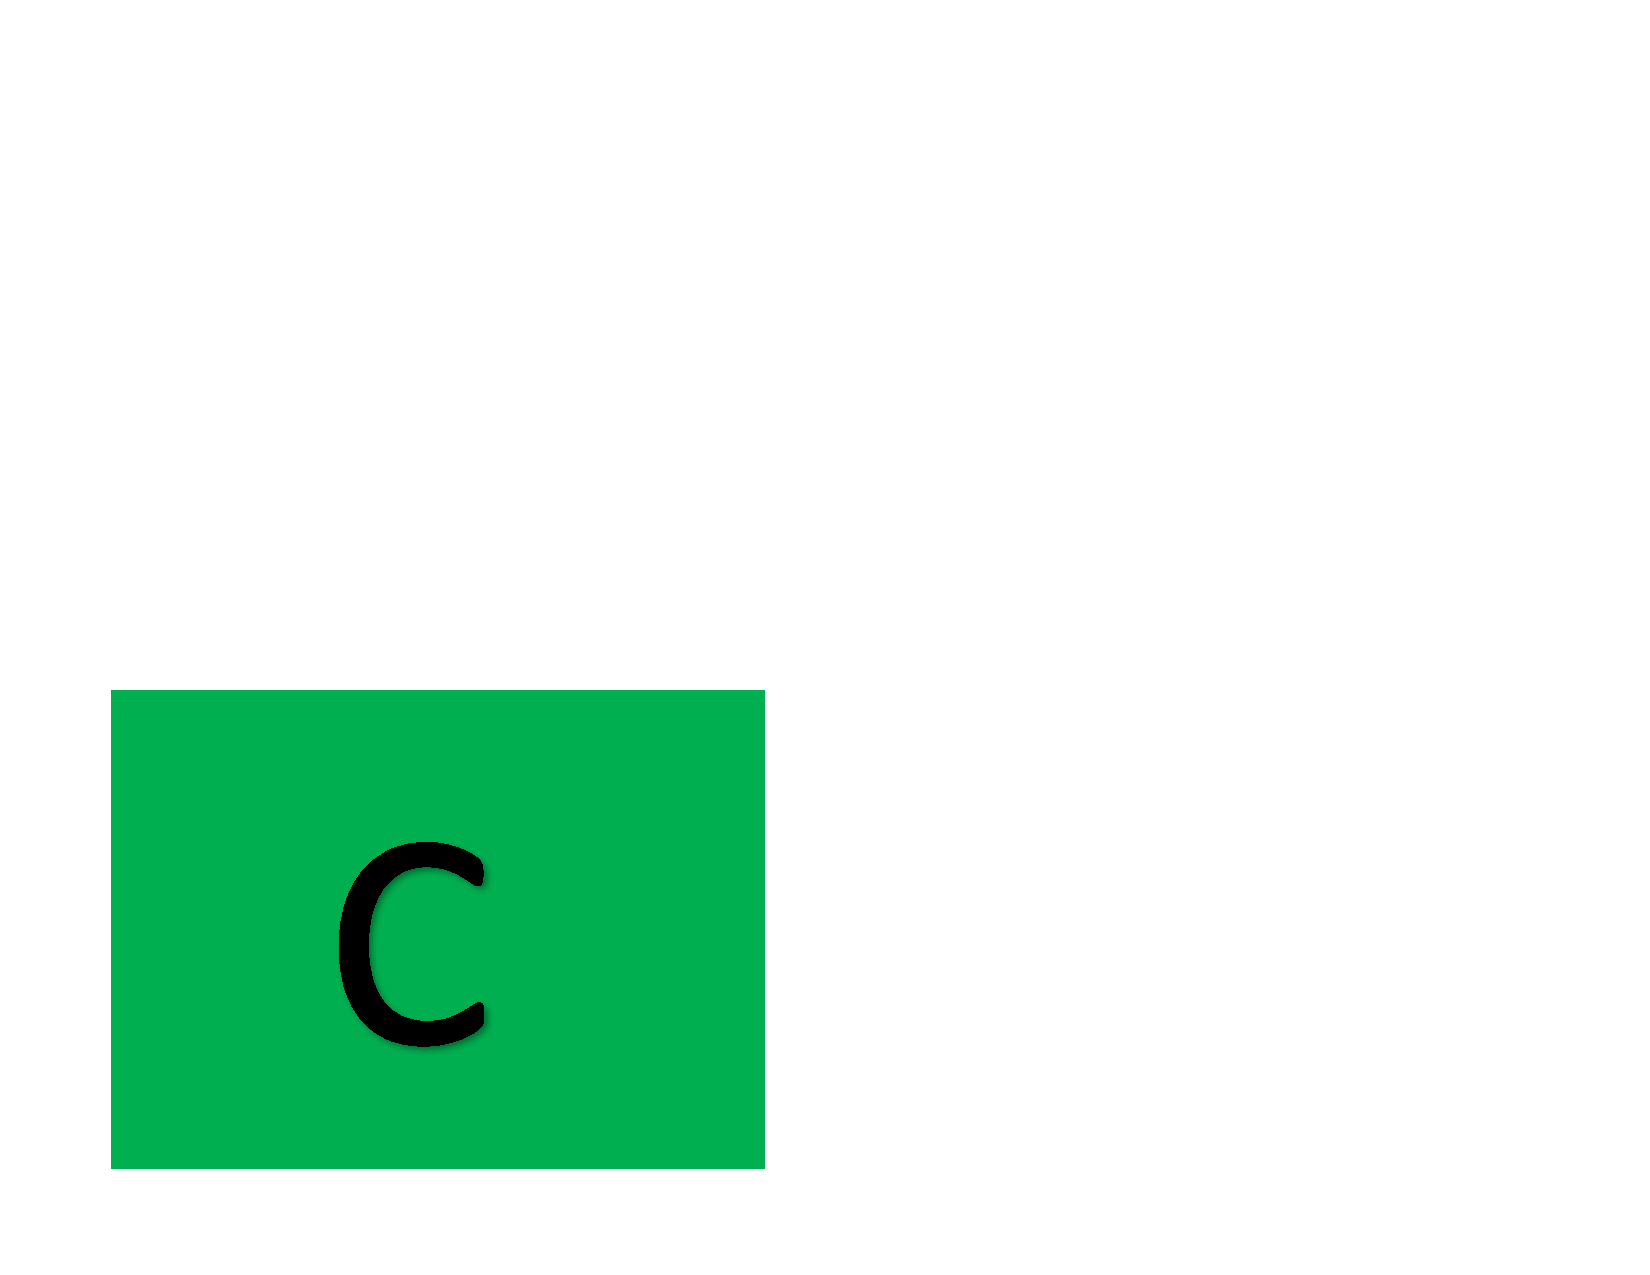
\includegraphics[width=0.8cm,height=0.5cm]{../../Lectures/figures/C}} ]  }
\newcommand*{\ditem}{ \item[{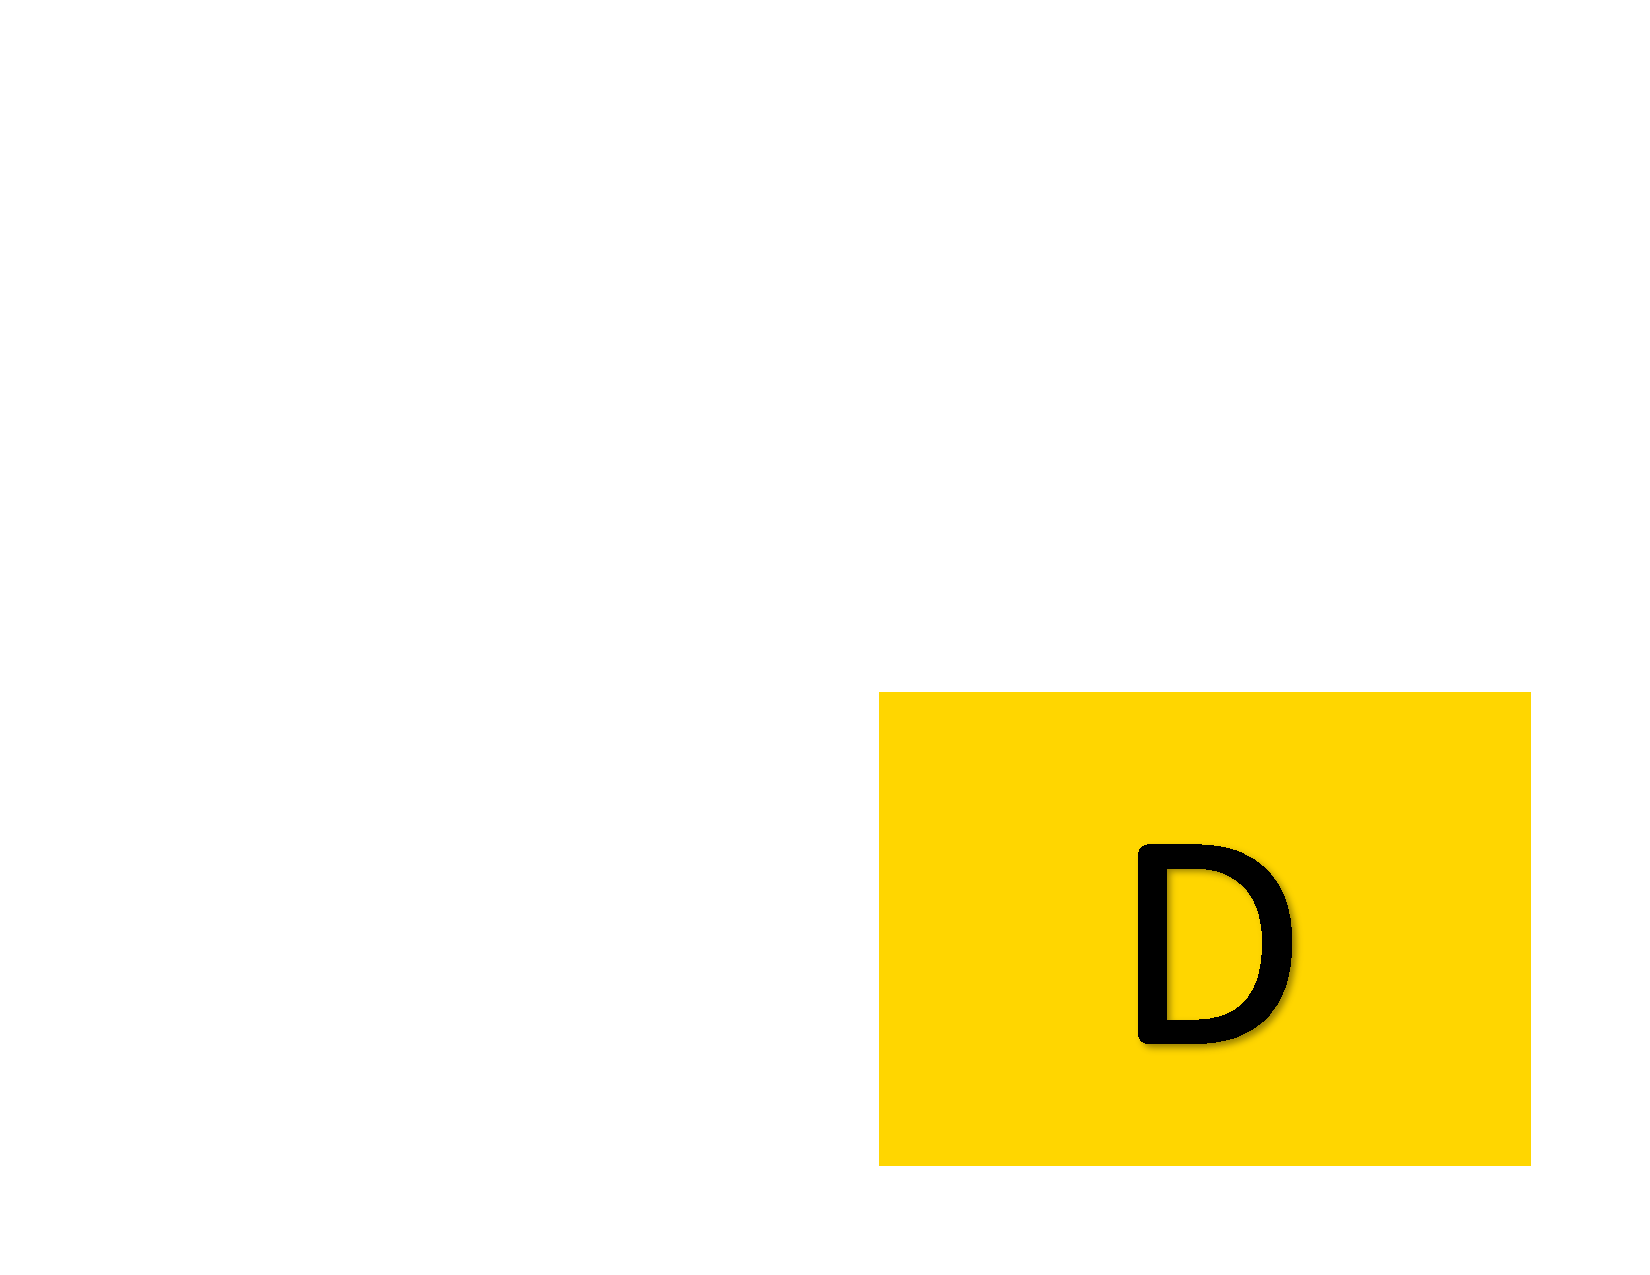
\includegraphics[width=0.8cm,height=0.5cm]{../../Lectures/figures/D}} ]  }
\newcommand*{\eitem}{ \item[{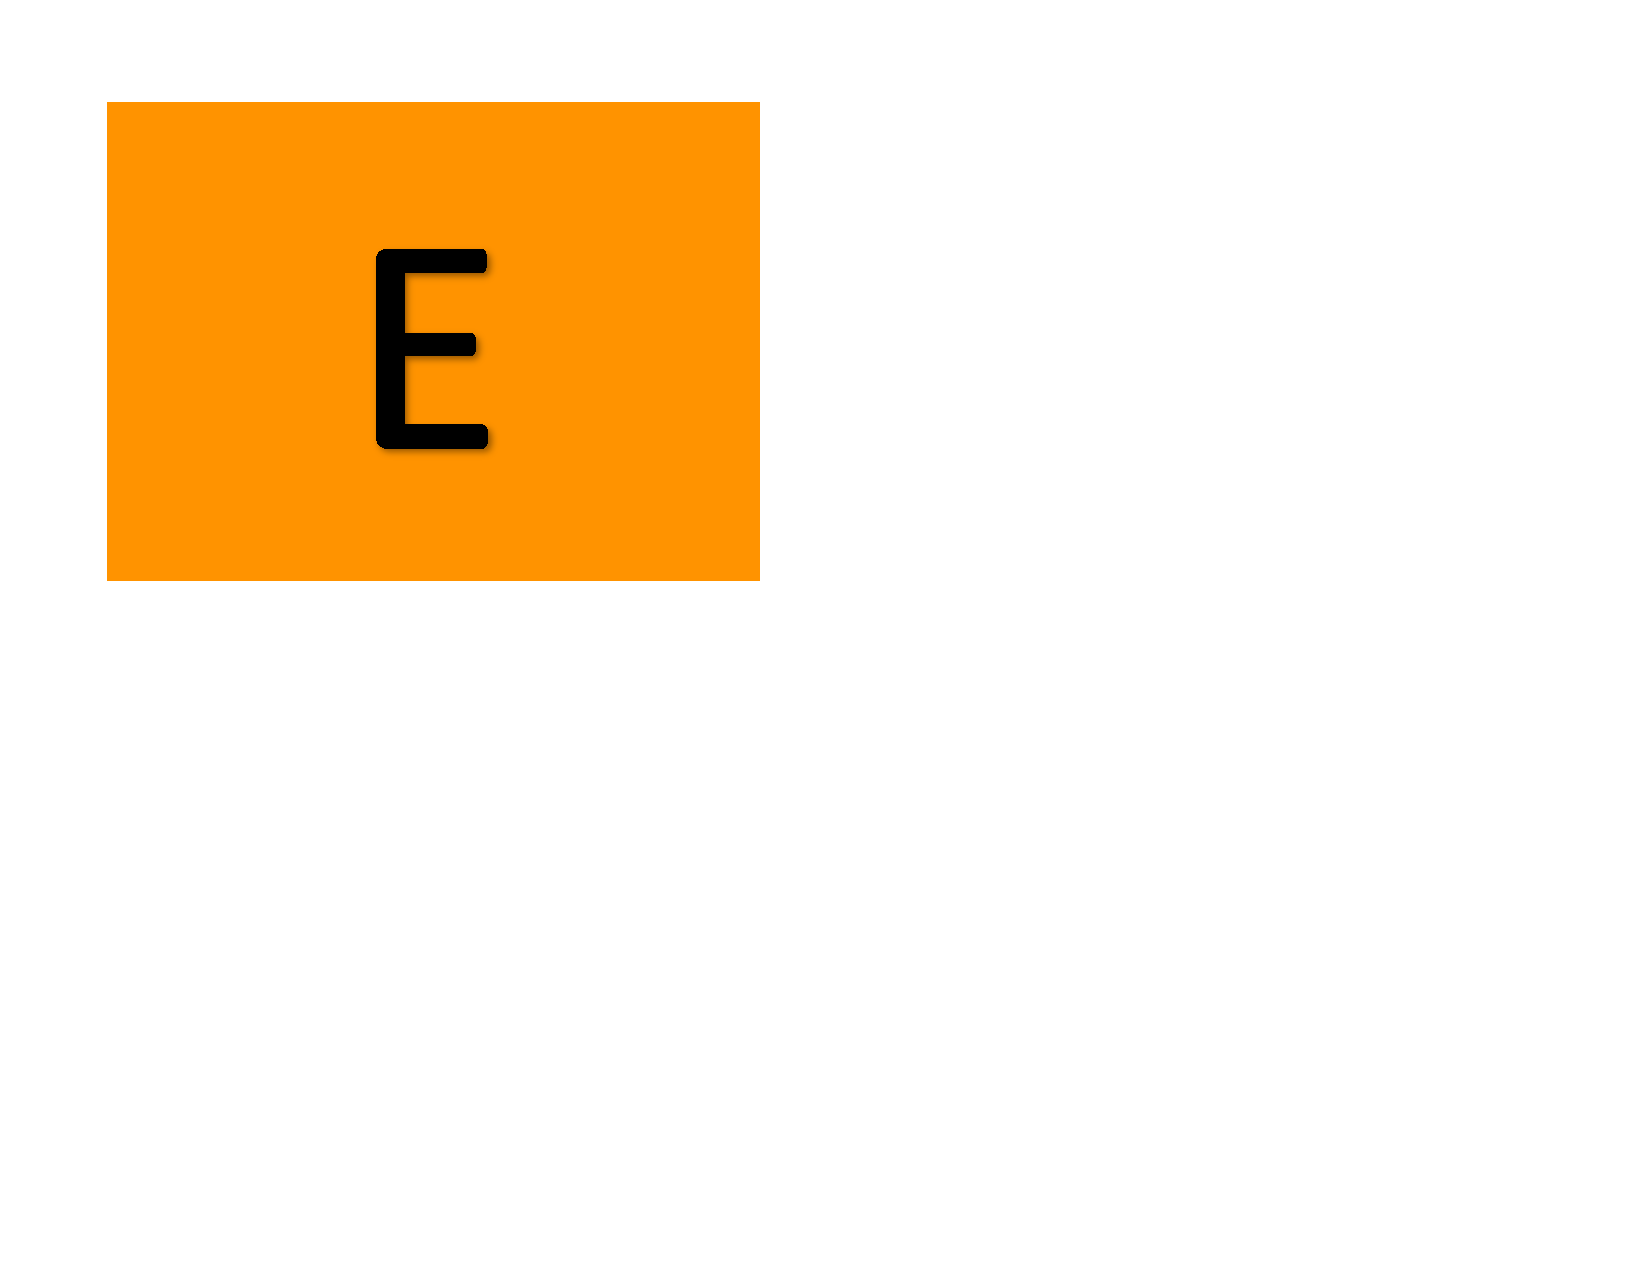
\includegraphics[width=0.8cm,height=0.5cm]{../../Lectures/figures/E}} ]  }
\newcommand*{\fitem}{ \item[{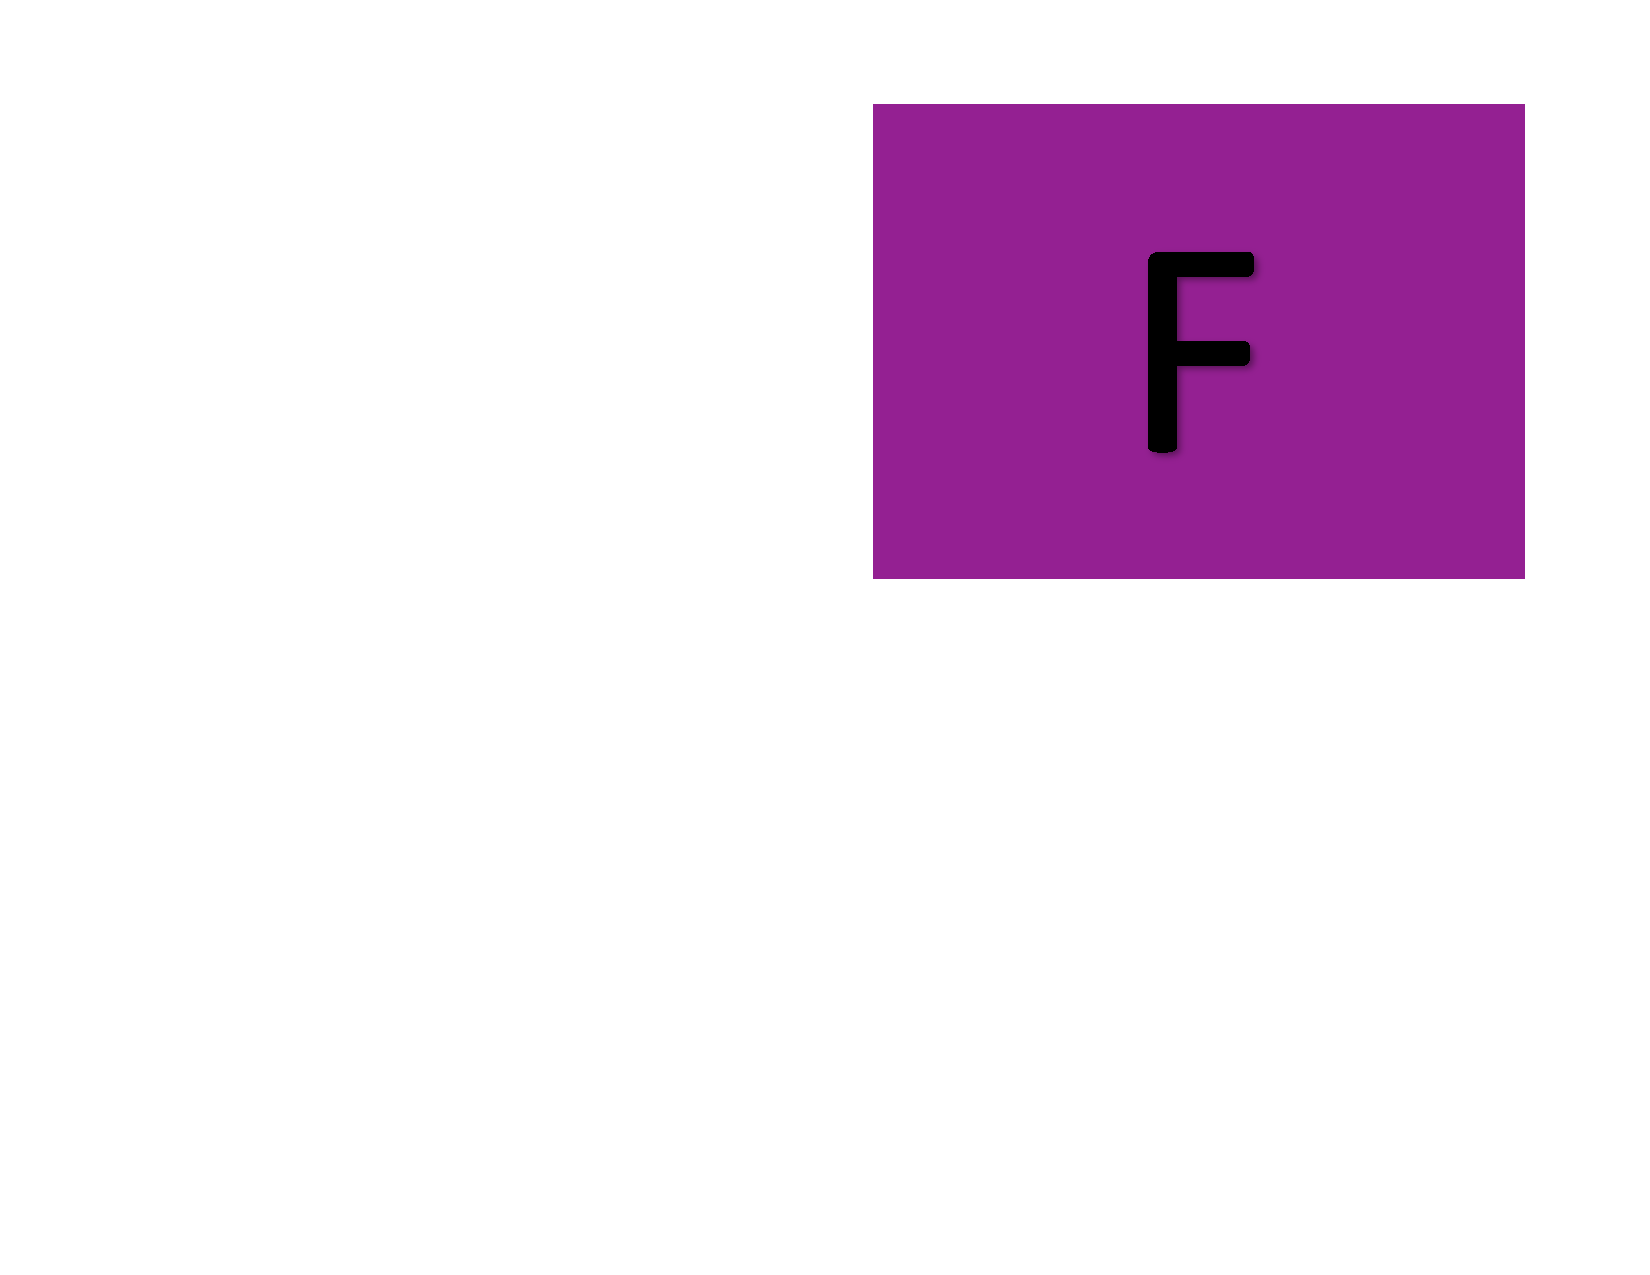
\includegraphics[width=0.8cm,height=0.5cm]{../../Lectures/figures/F}} ]  }


\newcommand{\hide}[1]{\underline{\phantom{#1 #1}}}

\usepackage{setspace}

\onehalfspacing
\usepackage{graphicx}

\begin{document}
\onehalfspacing

\lecture{1: Intro, Asymptotic Runtimes, Divide and Conquer}{January 14, 2025}

\paragraph{Course Logistics}

\begin{itemize}
\item Read section 2.3, and chapter 4 for first week of classes.
\item Read (or skim) chapters 1-3 to ensure familiarity with prerequisites
\item Syllabus quiz is due Sat, Jan 18. HW 1 and intro video due Fri, Jan 24
\end{itemize}

\section{Computational Problems and Algorithms}

\begin{definition} \noindent A \hide{\textbf{computational problem}} is a general task defined by a specific type of \hide{\textbf{input}} and an explanation for a desired \hide{\textbf{output}.} 
\end{definition}

\vs{.5cm}

\noindent A specific case of the problem is called an \hide{\emph{instance}.}

\begin{example}\textbf{Sorting} \\
\framebox{
\vbox{
\textbf{Input}: A sequence of $n$ numbers: $a_1, a_2, \hdots, a_n$
	
\textbf{Output:} A permutation $\sigma$ of the input sequence so that
	\begin{equation*}
	a_{\sigma(1)} \leq 	a_{\sigma(2)} \leq \cdots \leq 	a_{\sigma(n)}
	\end{equation*}
}}


An instance of this problem is the sequence %$1, 5, 92, -1, 2$.
\end{example}
\begin{example}\textbf{Min element} \\
	\framebox{
		\vbox{
			\textbf{Input}: An array of $n$ numbers: $[a_1, a_2, \hdots, a_n]$\\
			
			\textbf{Output:} The smallest element in the array and its index.
	}}
	
	\vs{5pt}
\end{example}

%\vs{1.5cm}
\begin{definition} \noindent An \textbf{algorithm} is a computational procedure that
	
	\begin{itemize}
		\item \hide{Takes in an input for a co}
		\item  \hide{Applies a concrete set o }
	\end{itemize}
	
An \textbf{algorithm} is said to be \textbf{correct} if it \hide{always produces }.
\end{definition}
\newpage


\section{Asymptotic Runtime Analysis (Chapter 3)}

\subsection{Rules for runtime analysis}
\begin{itemize}
		\setlength\itemsep{2em}
		\item $n$ denotes the size of the input
	\item Each basic operation takes constant time
	\item We focus on the \hide{worst case} runtime
	\item We only care about the \hide{order } of the runtime
\end{itemize}

\newpage
\subsection{Some initial examples}
\QU Given an array of $n$ items, find whether the array contains a negative number using the following steps:
\begin{algorithmic}
	\For{$i = 1$ to $n$}
	\If{$a_i < 0$}
	\State Return (true, $i$)
	\EndIf
	\EndFor
\end{algorithmic}
What is the runtime of this method?
\begin{enumerate}
	\aitem $O(1)$
	\bitem $O(n)$
	\citem $O(n^2)$
	\ditem It depends
	\eitem Other
	\fitem Don't know, I need a reminder for how this works.
\end{enumerate}
\end{Qu}

\vs{1cm}

\QU Given an $n \times n$ matrix $A$, what is the runtime of summing the upper triangular portion using the following algorithm? (same answers).
\begin{algorithmic}
	\State $\mathit{sum} = 0$
	\For{$i = 1$ to $n$}
	\For{$j = i$ to $n$}
	\State $\mathit{sum} = \mathit{sum} + a_{ij}$
	\EndFor
	\EndFor
	\State Return $\mathit{sum}$
\end{algorithmic}
\end{Qu}

\newpage
\subsection{Formal Definitions}
Let $n$ be input size, and let $f$ and $g$ be functions over $\mathbb{N}$.\\
\begin{definition}\textbf{Big $O$ notation}.\\
	
	A function $g(n) = O(f(n))$ (we say, ``$g$ is big-O of $f(n)$'') means:\\
	
	

\vs{3cm}
\end{definition}
\begin{definition}\textbf{Big $\Omega$ notation}.\\
	
	$g(n) = \Omega(f(n))$  means:\\
	
	\vs{3cm}
\end{definition}

\begin{definition}\textbf{$\Theta$ notation}.\\
	
	$g(n) = \Theta(f(n))$  means:\\
	
	\vs{3cm}
	
	
	Equivalently, this means 
	
\end{definition}
\newpage

\paragraph{Additional runtime examples}

\begin{enumerate}
	\item $4n^4 + n^3 \log n + 100n \log n$ \\ \\
	\item $n + 2(\log n)^2$ \\ \\
	\item $2^n + 10^{100} n^45$
\end{enumerate}


\vspace{2cm}

\paragraph{Logarithms in Runtimes}
Which of the following runtimes are the same asymptotically? Which are not?

\begin{itemize}
	\item $O(n \log n)$ and $O(n \lg n)$\\\\
	\item $O(\log n)$ and $O(\log^2 n)$\\\\
	\item $O(\log n)$ and $O(\log (n^2))$\\\\
	\item $O(n^{\log 100})$ and $O(n^{\lg 100})$\\
\end{itemize}
\newpage


\section{How to Present an Algorithm}
Presenting and analyzing can be broken up into four steps.
\begin{enumerate}
	\item \textbf{Explain}: the approach in basic English
	\item \textbf{Pseudocode}: for formally presenting the algorithmic steps
	\item {Prove}: the \textbf{correctness}
	\item {Analyze}: the \textbf{runtime complexity}
\end{enumerate}
As a rule it's a good idea to go through all steps when presenting an algorithm. Sometimes we will focus more on just a subset of these (e.g., you may be asked to prove a runtime complexity of an algorithm on a homework but not a correctness proof). \\ 


We will go through all four steps when we present the \emph{merge sort} algorithm.

\section{The Divide and Conquer Paradigm}

The divide and conquer paradigm has three components:
\begin{itemize}
	\setlength\itemsep{2em}
	\item \textbf{Divide}:
	\item \textbf{Conquer}:
	\item \textbf{Combine}:
\end{itemize}

\newpage

\paragraph{Example: Mergesort (Textbook, Chapter 2.3, 4)}
Given $n$ numbers to sort, apply the following steps:
\begin{itemize}
	\item Divide the sequence of length $n$ into %arrays of length $\ceil{n/2}$ and $\floor{n/2}$
	\item Recursively %sort the two halves
	\item Combine\\ %the two halves by merging
\end{itemize}

%\vs{6cm}
%\begin{figure}
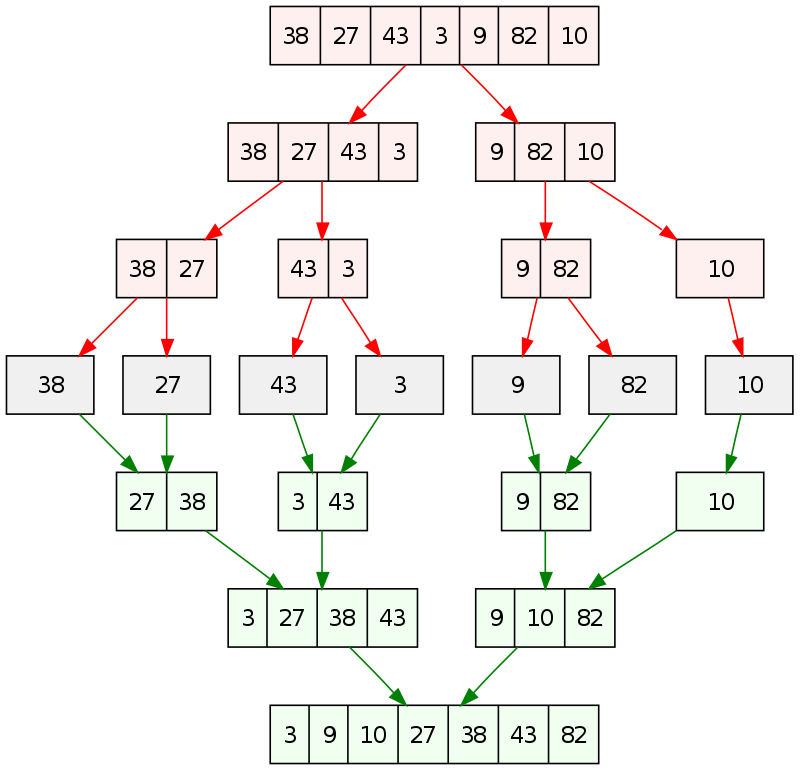
\includegraphics[width=.7\linewidth]{merge-sort.png}\\
%\end{figure}
Image courtesy of Wikipedia: \url{https://en.wikipedia.org/wiki/Merge_sort}.

%\paragraph{Pseudocode}
\begin{algorithm}
	$\textsc{MergeSort}(A)$ 
	\begin{algorithmic}
		\State $n = \textbf{length}(A)$
		\If{$n == 1$}
		\State %Return $A$
		\Else
		\State $m = \floor{n/2}$
		\State
		\State
		\State
		\State
		\State
	    \State
	    \State
		\State
		\EndIf
	\end{algorithmic}
\end{algorithm}


\newpage

\subsection{Analyzing The Merge Procedure}

%\vs{12cm}
\vfill
\textbf{Correctness:} To merge two sorted subarrays into a master array
\begin{itemize}
	\setlength\itemsep{2em}
	\item  Maintain a pointer to the \hide{end  of each subarray}
	\item  At each step, \hide{compare the two numbers from the end}
	\item Since subarrays are sorted, one of these numbers is \hide{guaranteed to be the} \\
	
	\hide{largest among unmerged numbers}
	\item so place \hide{that largest number in the next open} 
	\item At each step, we guarantee that: \hide{we place the next largest} \\
	
	\item So continuing until both subarrays are empty, \hide{this yields a sorted}
\end{itemize}

	
	
\end{document}
